

% \textbf{AL model}.
Мне было интересно посмотреть на поведение 2D системы для невзаимодействующего случая, в качестве начального состояния выбирался гауссов пакет, полностью лежащий в левой части системы, и также следил за контрастностью $I(t)$.  Наличие глобального гармонического потенциала описывалось слагаемым, вида $\sum_j u_j \hat{n}_j$. Эволюция считалась через ED (Exact Diagonalization) и разложением начального состояния по собственным (fig. \ref{fig:2Dtherm}a). Аналогично при небольшом уровне шума система термализовалась, а при больших значениях выходила на локализованное состояние.  

При термализующемся состоянии результат статзначим не зависит от начального состояния (результаты здесь не представлены). Интересно посмотреть на получающееся распределение заселенности узла $\langle n_j\rangle_t$, усредненное во времени, от энергии этого узла $\delta_j + u_j$ (fig. \ref{fig:2Dtherm}c). Также интересно сравнить $\langle n_j\rangle_t$ с получающимся термальным распределением $\tr n_j e^{-\beta H}$, коэффициент корреляции которых у меня получился 
\begin{equation*}
    \text{corr}\,(\langle n_j\rangle_t, \tr n_j e^{-\beta H})|_{\Delta=0.5}  \approx 0.8,
    \hspace{10 mm} 
    \text{corr}\,(\langle n_j\rangle_t, \tr n_j e^{-\beta H})|_{\Delta=5}  \approx 0.2,
\end{equation*}
что вполне соотносится с представлениями о локализации и термализации. 



 
\begin{figure}
    \centering
    \addletter{115}{a}
    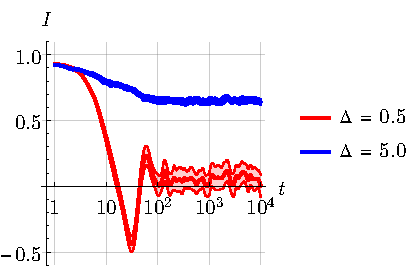
\includegraphics{imgs/2Dth_loc.pdf}
    % \hspace{5 mm} 
    \addletter{115}{b}
    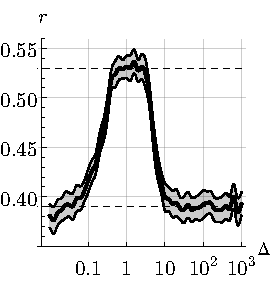
\includegraphics{imgs/2Drdel.pdf}
    % \hspace{5 mm} 
    \addletter{115}{c}
    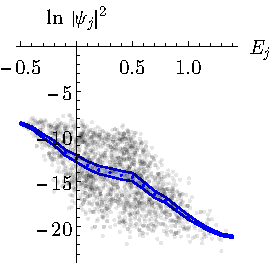
\includegraphics{imgs/2Dtherm_1.pdf}
    \caption{a) Эволюция контрастности $I(t)$, усреднённая по 50 реализациям $\delta_j$ для двух уровней шума $\Delta$: термализация и локализация. b) Зависимость $r$-parameter от уровня шума $\Delta$, усредненная по 50 реализациям $\delta_j$. c) Для термализованного состояния зависимость заселенности узла $|\psi_j|^2$ от энергии узла $E_j = \delta_j + u_j$, чёрными точками обозначена зависимость для конкретной реализации $\delta_j$, синим обозначен результат усреднения по 50 реализациям .}
    \label{fig:2Dtherm}
\end{figure}

Возникает естественный вопрос, каким именно образом можно охарактеризовать фазу локализации и ergodic phase (термализующуюся) системы, какому алгоритму можно скормить гамильтониан. Различные метрики представлены в \cite{pal_many-body_2010}, но лучше всего начать $r$-параметра, которому и посвящен следующий раздел. 








% experimental implementation of the model

